\chapter{Simulation and analysis tools}
The molecular dynamics workflow can be usefully divided as follows: 
\begin{enumerate}
\item Create initial condition
\item Run molecular dynamics
\item Analyze results
\end{enumerate}
Usually, step 3 will give experince that influence how steps 1 and 2 are done during the next iteration. It is important to have tools in place to accomodate this workflow. Most importantly, the tools have to be directly compatible when iterating $1 \to 2\to 3$. Otherwise, it is impossible to work efficiently. Second, it is convenient with compatibility $2\to 1$ if a simulation needs to be run furter in time. Third, it is convenient with compatibility $3 \to 1$, but the nature of such a compatibility is not as clear as the others. 



First choice is wheter to program the molecular dynamics simulator myself or to use a program made by someone else. I have implemented my own molecular dynamisc program before, and the experience from that tells me to use a package. It is quite easy to implement a simple molecular dynamics solver for Lennard-Jones particles in NVE and Berendsen NVT, but more complex potentials and barostatic ensembles are more challenging to implement and test. 

\section{LAMMPS}
Lammps, Large-scale Atomic/Molecular Massively Parallel Simulator, is a tool for (possibly) large particle-style simulations - mainly molecular dynamics. Lammps is a massive open source project, and its main features are developed and maintained at Sandia National Laboratories in the United States. 

From here follows a short introduction to practical use of Lammps. This section was written as memory notes to myself during the first month of using Lammps. 

\subsection{Input files}
Lammps input files are a set of commands to be executed. Some commands are only valid in the right order. The structure of such a file is:

\begin{enumerate}
\item \tb{Initialization:} Units, processors, boundary conditions, atom\_style, pair\_style
\item \tb{Atom definition:} Either from input file (restart/data) or making a lattice or region and create a box and atoms. 
\item \tb{Settings:} Typically thermostat and file dump information.
\item \tb{Run:} Choose number of timesteps.
\end{enumerate}
\paragraph{Example file}

\begin{lstlisting}[language=LammpsInput]
# ----------------- Init Section -----------------
units 			real
dimension 		3
boundary		p p p 
atom_style		full
pair_style		lj/cut/tip4p/long 1 2 1 1 0.1577 10.0
kspace_style	pppm/tip4p 1.0e-4
bond_style 		harmonic
angle_style		harmonic
pair_modify		mix arithmetic

# ----------------- Atom Definition Section -----------------
read_data "water_methane_test.data"

# ----------------- Settings Section -----------------
pair_coeff	1 	1 	0.21084 	3.1668
pair_coeff	2 	2	0.0 		0.0
pair_coeff	1 	2 	0.0 		0.0
bond_coeff  1 	0.0 0.9572
angle_coeff 1 	0.0 104.52
group water type 1 2
fix	fShakebond	water 	shake 	0.0001 100 0 a 1 b 1
pair_coeff 3 	3 	 0.29391 	3.73
group methane type 3
pair_coeff 	1 3 	0.18 	3.44
pair_coeff 	2 3 	0.0 	0.0

dump myDump all custom 5 output_x_barostat.lammpstrj id element x y z vx vy vz
dump_modify myDump element O H C

velocity all create 300.0 32352 rot yes mom yes dist gaussian
fix fxnpt all npt temp 300.0 300.0 100.0 x 400.0 400.0 100.0

# ----------------- Run Section -----------------
run   5000
\end{lstlisting}

Most properties are already set with a standard value, which means that only non-standard properties has to be set. 

\paragraph{atom\_style}
Atom style limits what kinds of interactions are possible to implement. For full flexibility, it is possible to set it to all.

\paragraph{pair\_style}
Pair style is the kind of interaction that are applied to all possible pairs of atoms. In practice, pair\_style sets all interations that are not part of specific bonded or angle interactions. 

\paragraph{bond\_style}

\paragraph{angle\_style}

\paragraph{pair\_coeff}

\paragraph{bond\_coeff}

\paragraph{angle\_coeff}


\subsubsection{Data files}
It is usually a good idea to have all atom input information i a file separate from the input file, and read it with the data\_read command. An atom data file shall contain positions and velocities for all particles. In addition, if some atoms are parts of specific molecules, this is decleared. All bonds and angles (and dihedrals and so on ..) that are meant to support interactions between specific particles must be decleared. In addition, it is possible to insert coefficients for the different interactions. However, it is not possible to declare atom\_style, pair\_style or any other style in the data files. This has to be done in the input file, and it is important that the number of coefficients in the data file is compatible with the interaction potential chosen in the input file. 

Below are some extractions from an input file for bulk water with bonded O-H interactions, and angular H-O-H interactions. I have used this file to simulate TIP4P water, by keeping the bonds and angles rigid with the shake-algorithm. 

\begin{lstlisting}[language=LammpsData]
LAMMPS data file via write_data, version 11 Nov 2013, timestep = 15000

10125 atoms
2 atom types
6750 bonds
1 bond types
3375 angles
1 angle types

-1.2998053548485800e-01 4.6629980535484322e+01 xlo xhi
-1.2998053548485800e-01 4.6629980535484322e+01 ylo yhi
-1.2998053548485800e-01 4.6629980535484322e+01 zlo zhi

Masses

1 1.00794
2 15.9994

PairIJ Coeffs

1 1 0 0 10
1 2 0 0 10
2 2 0.16275 3.16435 10

Bond Coeffs

1 0 0.9572

Angle Coeffs

1 0 104.52

Atoms

721 241 2 -1.0484400000000000e+00 -6.2221407531032169e-02 1.5159166496011423e+00 5.3069458514672112e+00 0 0 0
1396 466 2 -1.0484400000000000e+00 4.0240333910499935e+00 4.2356159167994916e+00 1.7598269969646658e+00 0 0 0
1398 466 1 5.2422000000000002e-01 4.7736723529825049e+00 3.6734646891601108e+00 1.9555433512796152e+00 0 0 0
718 240 2 -1.0484400000000000e+00 1.6591102071344288e+00 1.3108233273533909e-01 3.7368290353832792e+00 1 0 0
2115 705 1 5.2422000000000002e-01 2.6288644528128606e+00 1.8244264320027685e+00 3.9483095929557672e+00 1 0 0
.
.
.

Velocities

721 -5.0354515315883175e-04 5.3167587742950842e-03 3.3571203451087726e-03
1396 2.9628128063741773e-04 -3.6999987020118080e-03 -6.2672614595795321e-03
1398 1.9834410211762494e-03 -4.5261896434727186e-04 -3.5219356644226700e-03
718 6.4570329589514993e-04 -1.2753082693010263e-03 5.5441917429848477e-03
2115 1.9812407347396029e-03 -1.4861789372548064e-03 2.0816584325493676e-02
143 -7.7275724561505395e-03 1.4979358537740204e-03 1.9557938914574084e-02
720 -8.5445971109074596e-03 -1.7755485312369985e-02 1.4432539996760280e-02
2114 8.2504630257354671e-03 -1.5862538887645005e-02 1.1754578049979690e-02
722 1.8121516439040641e-02 -5.4646869701048756e-03 2.3672874162716955e-03
767 -7.7201655772992407e-03 -5.5203125867209482e-03 -1.2033511911111539e-02

.
.
.

Bonds

1 1 721 722
2 1 721 723
3 1 1396 1397
4 1 1396 1398
5 1 718 719
6 1 718 720

.
.
.

Angles

1 1 722 721 723
2 1 1397 1396 1398
3 1 719 718 720
4 1 9452 9451 9453
5 1 767 766 768
6 1 2114 2113 2115
7 1 53 52 54
8 1 143 142 144

\end{lstlisting}

This requires some explanation. The first lines are ignored by Lammps, so the first line to be interpreted is line 3. The first section, line 3-8, contains information about wat is supposed to be contained in this file. The next section defines the bounds on the simulation domain. Then comes a definition of the masses for the two atom types that were decleared in the first section. In the section called PairIJ Coeffs, parameters for pair\_style interactions are set. The last line in this section tells that pair\_style interactions between particles of type 2 and 2 in this simulations have parameters 0.16275, 3.1643 and 10. The first two parameters in the 1 1 and 1 2 interactions have value 0, which tells us that these don't interact pair\_style. The bond coefficient section decleares a bond with id 1. If there were to be additional types of bonded interactions, they would be numbered from 2 and so on. If the bond\_style is set to harmonic, the parameters for the first bond tells that the equilibrium distance in this harmonic bond is 0.9572, but that the coefficient for the harmonic force is 0. The reason for the coefficient to be zero in this specific case, is that the bond is to be rigid, and rigidity is handled later, by a fix-command. The angle coeffs section follows the same pattern as the bond coeffs. Th contents of the Atoms section can vary, depending on the atom\_style used in the simulation. This setup is for atom\_style full. Line 35 tells that atom number 721 belongs to molecule number 241. It is of type 2 (oxygen in this case), and has charge -1.04844. Then comes xyz positions, and an nx ny nz counter telling how many times the atom has passed each periodic wall. Velocities are self-explanatory. The bonds section lists all the bonds that are defined in the simulation. In this case it is O-H-bonds in water. line 63 tells that the first such bond is of type 1 (as defined in bond coeffs), and that it creates a bonded interaction between atoms 721 and 722. The angles section is similar, but it takes three atoms to make an angle, with the vertex in the middle. This type of declaration is quite powerful. We have only defined that we have some water molecules, and that they support bonded and angular interactions, as well as pair\_style interactions. That means we can use any potential (supported by lammps) that have these restrictions. The only thing that has to be changed, are the coefficients for the different interactions. If one wishes to change potentials regularly, it can be a good idea to put coefficients in a file together with the declaration of potentials, using the {\tt $<$pair, bond, angle$>$\_coeff } commands. 



\subsection{Interaction Potentials}

\subsection{Settings}
\subsubsection{The fix command}

\subsection{Computes in lammps}
\subsubsection{Pressure}
LAMMPS calculates the symmetric stress tensor for the system during each timestep, and stores it as a 6-element vector. The formula used for caculation is:
\begin{equation}
	P_{ij} = \frac{\sum_k^N  m_k v_{ki} v_{kj}}{V} + \frac{\sum_k^N r_{ki} f_{kj}}{V}
\end{equation}
Rigid sets of atoms with the SHAKE algorith are accounted in this calculation. In practice, fix SHAKE adds forces to the atoms before integration to account for their holonomic constraints. These forces are included in the virial when calculating the pressure. 


All commands are available from the LAMMPS documentation \cite{lammps:input_commands}. A very good beginners guide for LAMMPS \cite{lammps:guide:pittsburg}

\section{Optimizations in LAMMPS}
\subsection{OpenMP}
OpenMP support is implemented in the USER-OMP package. This has turned out not to be entirely stable. (Random crashes with cannot compute pppm)
\subsection{Processor layout and partitions}
{\tt run\_style verlet/split} distributes force calculations over two partitions of processors. These partitions must be defined either using the {\tt processor} command or the {\tt partition} command. {\tt verlet\_split} depends on the REPLICA package. 


\section{Extending LAMMPS}
LAMMPS was designed to be easily extendable, and in my opinion that turns out to be true.

I have made @number extension to LAMMPS.

\subsection{Region {\tt eprism} -- elliptical prism}
\label{subsec:reg_eprism}
I have written a simple extension to LAMMPS, which enables med to define regions formed like elliptical prisms. This is needed to carve out elliptical holes for my simulations. 

The main contents of this extension is:

\begin{lstlisting}[language=c++]
int RegEprism::inside(double x, double y, double z) 
{
	double dx = x-xmid;
	double dy = y-ymid;
	return ( (dx/a)*(dx/a)+(dy/b)*(dy/b) ) < 1.0;
}
\end{lstlisting}

The extension is a class that inherits from {\tt class Region}. 
From the class definition of class region it can be seen that its subclasses are required to implement three functions:

\begin{lstlisting}[language=c++]
virtual int inside(double, double, double) = 0;
virtual int surface_interior(double *, double) = 0;
virtual int surface_exterior(double *, double) = 0;
\end{lstlisting}

I was not going to use the surface functions, so I only needed to implement {\tt inside(...)}. I left the other two as dummy functions returning {\tt false}. Using this region with LAMMPS functionality that requires knowledge of the region surface can result in undefined behavior.


\section{General Utility Lattice Program}
It is cumbersome to calculate stiffness paramenters using molecular dynamics. Therefore I use a dedicated program -- General Utility Lattice Program (GULP) -- to caculate these parameters. @IProbablyWontUseGulpForTheMaster

\section{Crack tracer}
Measuring the area of a crack surface is far from a trivial task. Due to the fractal-like interface between a molecular surface and the ``void'', at least one adjustable parameters must be included in a method for calculating the surface are of a crack in a molecular system. One possibility is to measure the solvent-accessible area, which has \emph{one} free parameter: The radius of a trial particle rolling over the molecular surface. 


\subsection{Algorithm}
I have implemented a Monte-Carlo crack tracer based on the theory of @cite1970isj to measure the solvent-accessible area of a system of particles. The basic idea is that every point in space is defined as either part of the \emph{void} or part of the \emph{wall} based on the following definition: A void point is a point for which there exist no particles within a distance $r_p$. Points that are not part of the void are parts of the wall. The Monte-Carlo method I employ is as follows: $N$ line segments of length $\Delta l$ and uniformly random orientation and position in space are drawn. A surface point is detected if one of the edges is in the void while the other is in the wall, and is identified as the midpoint of the line segment. The solvent-accessible surface area of the system is then, based on @cite1971:

\begin{equation}
A_{ss}(r_p) = 2V\frac{n_s(r_p)}{N\Delta l}
\end{equation}

Where $n_s$ is the number of surface points detected amond $N$ line segments. $V$ is the volume of the system. The length $\Delta l$ is the only numerical resolution parameter for this measure, and has to be small compared to $r_p$ in order to capture the surface structure. 

\subsection{Implementation}
\paragraph{Cell lists}
The system is divided into a maximum number of equal sized cells such that that all cell dimensions $l_x, l_y, l_z$ are greater than $r_p$. When a point is checked for whether it is part of the void or the wall, only the distance to particles belonging to the same cell and the directly and diagonally adjacent cells needs to be checked. Using cell lists rather that looping over all particles in the system gives huge efficiency gains.
\paragraph{Periodic boundaries}
Periodic boundaries are implemented using cell lists, which means that the system must be at least $2\times 2 \times 2$ cells – each dimension in the system must be at least $2r_p$.
\paragraph{Scaling efficiency}
If we assume that the required number of samples to estimate the surface area of a system is proportional to the number of particles in that system, the problem scales as $\mathcal{O}(N^2)$. With cell lists the problem scales like $\mathcal{O}(N)$.


\section{Stress measurement (crude)}
I output the stress tensor for each particle averaged over @Ndump steps. These values are put on a 2D grid, and averaged for each cell on that grid. This kind of measurement is not necessarily useful for methane hydrates, as the characteristic size is large (12 Å) so that the grid must necessarily be coarse. @IsThisTrue?@TurnsOutToBetrue. It actually turns out that i get the best results by using the same number of grid points as there are unit cells in each direction. This is close to averaging over each unit cell, which should give units that are comparable. Slightly lower or higher resolutions of the grid give artifacts @insertfigure and much higher resolutions results in very few atoms contributing to each grid cell, which gives bad statistics and useless results. 

\begin{figure}
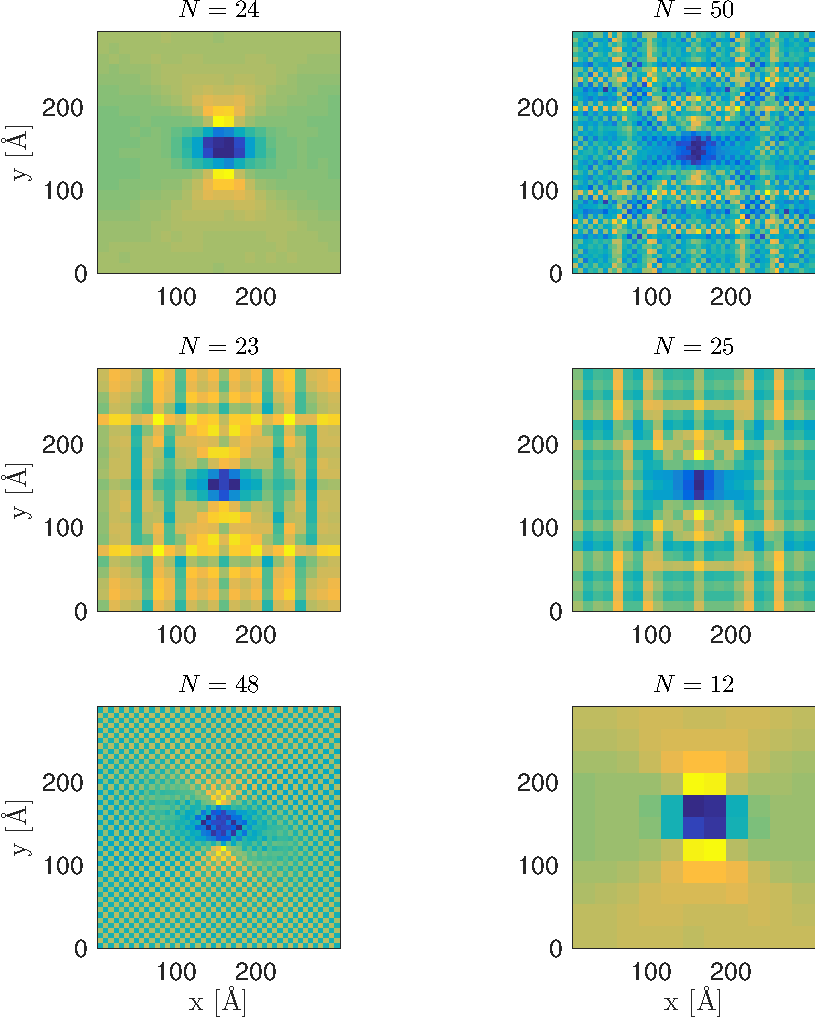
\includegraphics[width=\textwidth]{../figures/thesis/stressfield_artefacts.pdf}
\caption{Measured stress fields in the xy-plane with different resolutions of the cell grid. The modeled system is $24\times 24\times 12$ S1 unit cells. We see that $N=24$ and $N=12$ works well. $N=48$ gives a checkered pattern, but it is possible to see the stress field. The hichest resolution available without ertefacts is the number of unit cells in each direction.}
\end{figure}